\section{Physical Threat Model}\label{sec:phys}

The recovery calculus is meaningful only against a physically grounded
model of perturbation. This section establishes that ground.
We separate three concerns: the taxonomy of Single-Event Effects
(\ref{sub:see}), the layer-specific physics of volatile memory
(\ref{sub:dram-sram}), and the layer-specific physics of NAND-flash
persistent memory (\ref{sub:nand}). A consolidated view appears in
\cref{tab:layer-physics}. Emerging technologies are positioned
in~\ref{sub:emerging}.

\subsection{Single-Event Effects: Canonical Taxonomy}\label{sub:see}

Following~\cite{dodd2003,baumann2005,jedec89a}, we adopt the standard
SEE classification:

\begin{itemize}
\item \textbf{SEU} -- Single-Event Upset. A single bit (or a few
  adjacent bits in a contiguous physical layout) transitions
  state under the charge deposited by an ionizing particle.
\item \textbf{MBU} -- Multi-Bit Upset. Two or more bits in the same
  logical word change state from a single particle event,
  typically because the particle's track ionizes adjacent cells.
\item \textbf{SET} -- Single-Event Transient. A transient voltage
  pulse on a combinational logic path. May propagate to a latch and
  become an SEU, or may dissipate before the next clock edge.
\item \textbf{SEFI} -- Single-Event Functional Interrupt. A
  particle-induced state corruption of a control register or finite
  state machine that puts a sub-system into a non-functional state
  recoverable only by reset.
\item \textbf{SEL} -- Single-Event Latchup. A parasitic thyristor
  structure activates, causing a destructive over-current condition
  unless promptly mitigated~\cite{normand1996}. Catastrophic
  without hardware support; outside this report's scope.
\end{itemize}

For the purposes of BEAMFS, the relevant subset is~\(\{\mathrm{SEU},
\mathrm{MBU}\}\) acting on memory cells, and~\(\{\mathrm{SET}\}\) acting
on the bus and DMA paths between memory and CPU. SEFI and SEL are
hardware-recovery problems (watchdog reset, power cycling), modelled
here only as the boundary~\(\bot\).

The probability of an SEU striking a given memory cell exposed to a
particle flux~\(\Phi\) (particles\,cm\(^{-2}\)\,s\(^{-1}\)) of linear
energy transfer~\(\mathrm{LET}\) (MeV\,cm\(^2\)/mg) is, to first order,
the product of flux, integrated cross-section, and exposure time
\cite{petersen1996}:
\begin{equation}
  P_{\text{SEU}}(\text{cell}, t) = 1 - \exp\!\bigl(-\sigma(\mathrm{LET})\,
  \Phi \, t\bigr),
  \label{eq:seu-prob}
\end{equation}
where~\(\sigma(\mathrm{LET})\) is the SEU cross-section curve of the
specific cell technology, conventionally measured in
cm\(^2\)/bit. \Cref{fig:see-cross-section} reproduces typical
cross-section curves for the three technology classes treated in
this report, derived from the canonical reviews
\cite{dodd2003,baumann2005,cai2017nand}.

\begin{figure}[t]
\centering
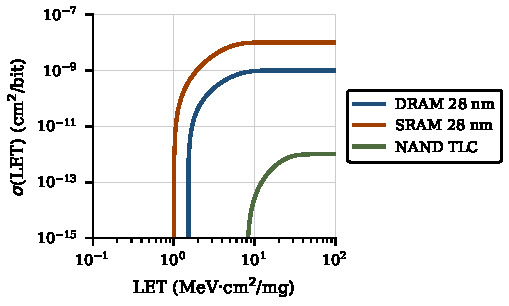
\includegraphics[width=\columnwidth]{figures/fig1.pdf}
\caption{SEE cross-section curves for three memory-stack layers, fit
to a Weibull form
\(\sigma(\mathrm{LET}) = \sigma_{\mathrm{sat}}\,
\bigl[1 - \exp(-((\mathrm{LET}-L_{0})/W)^{s})\bigr]\)
with onset threshold~\(L_{0}\) and saturation~\(\sigma_{\mathrm{sat}}\).
Weibull parameters are taken from canonical reviews
\cite{dodd2003,baumann2005,cai2017nand}; see~\cref{tab:layer-physics}
for typical FIT rates per technology.}
\label{fig:see-cross-section}
\end{figure}
\FloatBarrier

\begin{remark}
\Cref{eq:seu-prob} is a single-cell, time-independent first-order
model. It ignores temperature dependence, voltage scaling, and
inter-cell correlation. We use it to size orders of magnitude only;
the recovery operator's soundness does \emph{not} rely on its
quantitative accuracy. Real device cross-sections exhibit
Weibull-shaped curves with onset threshold and
saturation~\cite{petersen1996}; the figures use Weibull fits, while
the body retains the simple exponential form for clarity.
\end{remark}

\subsection{Volatile Memory: DRAM and SRAM}\label{sub:dram-sram}

\paragraph{DRAM.}
Dynamic random-access memory stores each bit as charge on a single
capacitor controlled by a single transistor (1T1C cell). The charge
naturally decays and must be refreshed every \(\sim\)64\,ms. Two
phenomena make DRAM cells SEU-vulnerable:
\begin{itemize}
\item Particle strikes deposit charge that adds to or subtracts from
  the stored capacitor charge. Above a critical
  charge~\(Q_{\text{crit}}\) (\(\sim\)10\,fC for DRAM cells, an
  order of magnitude above the \(\sim\)1\,fC range of bistable SRAM
  latches~\cite{baumann2005}), the cell flips state.
\item As the technology node shrinks, the cell's capacitance and
  thus~\(Q_{\text{crit}}\) decrease. Per-bit SEU sensitivity therefore
  rises with miniaturization, partially offset by smaller geometric
  cross-section.
\end{itemize}

A modern DDR5 module ships with on-die ECC~\cite{jedec79-5}, which
silently corrects single-bit errors within the chip. The error
stream visible to the kernel is therefore a \emph{filtered} version
of the raw cell event stream. In v1 of this report we model the
unfiltered matrix; on-die ECC is treated as a strengthening assumption
to be added in v2. The recovery operator's soundness
theorem (\cref{thm:soundness}) is constructed so that any cell-level
filter applied upstream of the kernel can only \emph{decrease} the
residual event rate seen by BEAMFS, never increase it.

\paragraph{SRAM.}
Static RAM (CPU caches, FPGA configuration memory) uses a six-transistor
bistable cell. Particle strikes induce SEU by upsetting the bistable
latch when the deposited charge exceeds the latch's noise margin.
SRAM is more SEU-sensitive per cell than DRAM at modern
nodes~\cite{dodd2003,baumann2005}: typical sea-level FIT rates are
\(\sim 10^{3}\) FIT/Mbit for SRAM versus \(\sim 10^{-3}\) FIT/Mbit
for DRAM, a six-orders-of-magnitude gap explained by the smaller
critical charge of bistable latches compared with capacitors.
SET pulses on combinational paths can propagate into SRAM latches
at the next clock edge. CPU caches with parity or ECC partially
mitigate this; older or embedded CPUs without cache ECC remain
vulnerable. The kernel's exposure to SRAM SEU is indirect (data
transits the cache before being written to DRAM); BEAMFS treats
this as part of the volatile-memory layer for purposes of the
recovery calculus.

\subsection{NAND Flash via NVMe: Cumulative Mechanisms}\label{sub:nand}

NAND-flash storage stores bits as trapped charge on a floating gate.
The energy required to flip a NAND cell with a single particle event
is high enough that direct SEU on NAND is rare~\cite{cai2017nand,
mielke2017}. The dominant failure modes are cumulative:
\begin{itemize}
\item Program/Erase (P/E) cycle wear, leading to retention loss.
\item Read disturb, where repeated reads of one page perturb adjacent
  pages.
\item Retention loss over time, accelerated by temperature and prior
  P/E count.
\end{itemize}

These are not Single-Event Effects in the strict sense; they are
TID-related and use-related cumulative effects. They do however
interact with the recovery calculus, because the persistent layer's
contribution to the filesystem state can itself become inconsistent
over time even without any radiation event. BEAMFS v1 models the NAND
layer's expected error rate as a function of P/E cycles and retention
age, following the empirical model of Cai \emph{et al.}~\cite{cai2017nand}
and Mielke \emph{et al.}~\cite{mielke2017}, calibrated to the JEDEC
endurance specification~\cite{jedec218b}.
\Cref{fig:nand-retention} shows the expected raw bit-error rate of
typical TLC NAND as a function of retention time across three P/E
states.

\begin{figure}[t]
\centering
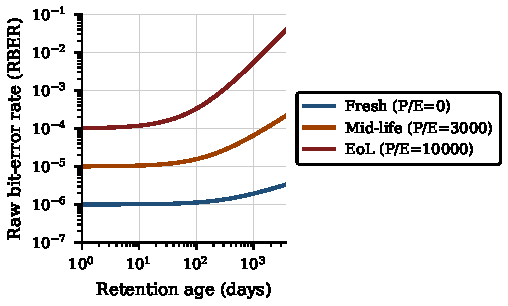
\includegraphics[width=\columnwidth]{figures/fig2.pdf}
\caption{TLC NAND raw bit-error rate (RBER) as a function of retention
age, parameterized by P/E cycle count. Empirical model derived
from~\cite{cai2017nand,mielke2017}; values at end-of-life and 1-year
retention align with the JEDEC JESD218B endurance
specification~\cite{jedec218b} (raw BER \(\sim 10^{-3}\) at EoL,
post-LDPC UBER \(\le 10^{-15}\)). The cumulative drift visible at
high P/E distinguishes NAND from the volatile-layer SEU regime
of~\cref{fig:see-cross-section}.}
\label{fig:nand-retention}
\end{figure}
\FloatBarrier

The recovery operator must therefore handle two distinct error
populations on the persistent side: (i) rare direct SEU, treated
identically to volatile-layer events, and (ii) NAND-cumulative
errors, treated as a slowly varying background that the operator
must remain stable against, not correct against (correction is the
job of the SSD's internal LDPC engine, below the filesystem).

\subsection{Emerging Technologies}\label{sub:emerging}

3D XPoint (Optane) was a phase-change memory whose development was
discontinued in 2022; we mention it for completeness only.
Resistive RAM (ReRAM) and Magnetic RAM (MRAM) are emerging
non-volatile technologies with substantially different failure
modes: ReRAM is largely insensitive to SEU but vulnerable to
filament instability; MRAM is largely insensitive to ionizing
radiation but vulnerable to external magnetic fields. v1 of this
report does not model them; their integration into BEAMFS would
be a v3-or-beyond consideration, and the recovery operator's
generic structure (\cref{sec:m2c}) is designed not to forbid
their later inclusion.

\subsection{Consolidated Layer View}\label{sub:layer-table}

\Cref{tab:layer-physics} summarizes the dominant failure mode per
layer, the relevant order-of-magnitude rates from canonical sources,
and the recovery-relevant exposure for BEAMFS. The numerical
values are deliberately rounded to one or two significant figures;
the canonical sources cited in each row provide tighter values
where required.

\begin{table*}[t]
\centering\small
\caption{Memory-stack layers, dominant failure modes, and order-of-magnitude
rates. Values are taken as canonical reference points from the cited
literature and are rounded to one significant figure; see those
sources for tighter, technology-specific numbers. FIT denotes
``failures in time'', \(\mathrm{1\,FIT} = \mathrm{1}\) failure per
\(10^{9}\) device-hours.}
\label{tab:layer-physics}
\begin{tabularx}{\textwidth}{l X l X}
\toprule
\textbf{Layer} & \textbf{Dominant failure mode} & \textbf{Reference rate} & \textbf{Source} \\
\midrule
DRAM (28~nm)  & SEU on capacitor cell, MBU on physically adjacent cells &
\(\sim 10^{-3}\)~FIT/Mbit at sea level &
\cite{baumann2005,jedec89a} \\
\addlinespace[0.3em]
SRAM (28~nm) & SEU on bistable cell, SET on combinational logic &
\(\sim 10^{3}\)~FIT/Mbit at sea level (six orders of magnitude above DRAM) &
\cite{dodd2003,baumann2005} \\
\addlinespace[0.3em]
NAND (TLC, 3D 232L) & Cumulative retention loss; rare direct SEU &
\(\sim 10^{-3}\)~raw BER at EoL P/E + 1\,year retention &
\cite{cai2017nand,mielke2017,jedec218b} \\
\addlinespace[0.3em]
DDR5 on-die ECC      & As DRAM, with on-chip single-bit correction & filtered DRAM rate (visible undetected event rate substantially reduced) &
\cite{jedec79-5} \\
\bottomrule
\end{tabularx}
\end{table*}

The vertical separation of these layers, and the qualitatively
different physics of each, motivate the multi-layer structure of
the state space defined in~\cref{sec:state}.
